\section{Phase-Scoped Implementation and Qualification (RQ2)}
\label{sec:repair}
\subsection{Constraining attention while retaining batched work}
The RTX candidate changes the non-flash Qwen3 attention subgraph inside \texttt{build\_attn\_mha}. An initial implementation constructs one attention subgraph per query and concatenates the results. A subsequent implementation represents query columns in the ggml batch dimension, allowing existing operations to process them in parallel while retaining a one-column query structure. Projection, output projection and feed-forward computation remain batched. The change is local to the graph representation, rather than global UB1 execution of every operation.

After the existing query/key/value permutations, the query tensor has dimensions $(d,q,h,1)$ in the supported single-KV-stream case. The candidate uses \texttt{ggml\_view\_4d} to reinterpret it as $(d,1,h,q)$, preserving the source strides and using the original query-column stride for the new batch axis. The attention mask similarly changes from a query-column layout to $(n_{\mathrm{KV}},1,1,q)$. Existing key-query multiplication, softmax, value multiplication and final contiguous recombination remain in the non-flash graph. Shared K/V tensors are not reconstructed from a reference answer. The purpose is to retain the tested scalar-query computation structure while preserving parallel execution elsewhere.

The source explicitly restricts this branch to Qwen3, non-flash attention, one KV stream, compatible mask dimensions, and absent attention bias, sinks and MLA value projection. The initial query limit is four; a source-bound later width build raises that assertion to eight without changing backend arithmetic. These guards define the implemented family. They do not establish invariance for every model graph, precision, shape or backend. Native output qualification supplies the behavioral evidence.

\subsection{Phase dispatch and graph reuse are part of the implementation}
The scope mask is process-fixed. A thread-local guard selects one of four bits by model role and by whether the call is prefill or continuation: target bits 1/2 and draft bits 4/8. It restores the prior active state on exit. The guard executes before the capture-disabled fast path returns to native \texttt{llama\_decode}, so disabling diagnostic metadata does not disable the constraint.

The selected boolean is copied into graph parameters and graph context. Graph reuse is rejected when that boolean differs from the cached topology key. This prevents a graph constructed for one phase layout from being reused solely because the ordinary microbatch fields match. The server also resets the phase to prefill when starting a new prompt. Scope selection is therefore an actual dispatch and reuse condition, rather than a label attached after execution.

Capture-disabled costs bypass observer metadata construction and forced observer synchronization. Qualification separately checks captured multi-query nodes and capture-on/off behavior. The source also contains a conditional target-state move after the first pending sample; the expansion environment does not set its activating continuation-UB variable. The measured RTX candidate consequently pays for native drafting, verification and reconciliation, but no state transplant is inferred merely from the presence of that branch. S1 and S2 bind the relevant patch files and timer audit.

\subsection{The finite phase family}
Figure~\ref{fig:phase} presents the full four-switch factorial: 16 masks, four exposed HumanEval probes and two repetitions, totaling 128 requests. All outputs and registered stop boundaries are repeat-stable. Masks 3, 7, 11 and 15 pass the complete probe panel. /15 and /31 pass every mask; /25 needs at least one target-phase bit; /18 needs both target phases. Draft-phase bits do not change this pattern.

\begin{figure}[!htbp]
\centering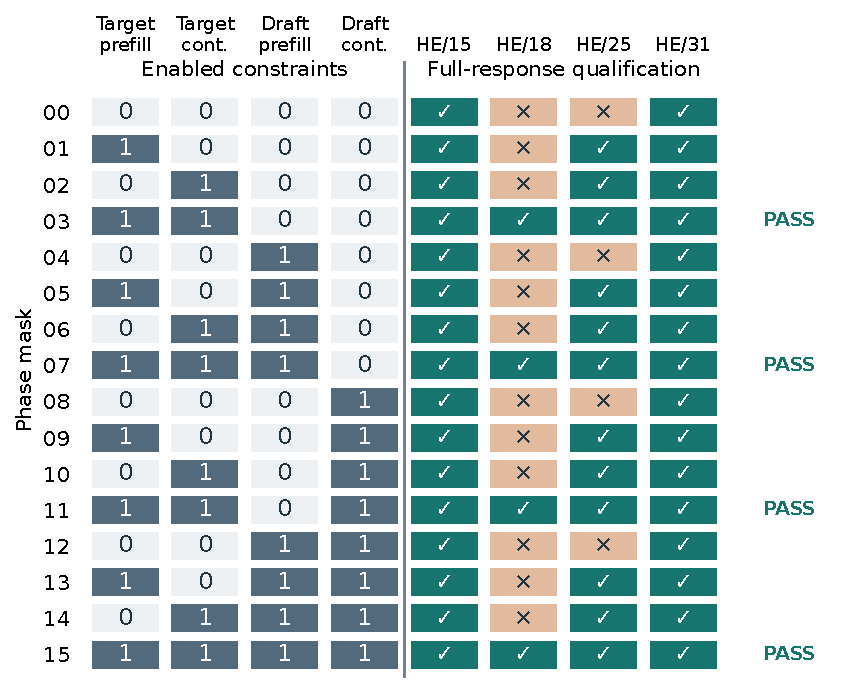
\includegraphics[width=\linewidth]{figures/figure_3_phase_matrix.pdf}
\caption{RTX phase qualification at fixed $k=3$, UB4 and cap128. Left columns show enabled phase bits; right columns show native full-response qualification for each probe in both repetitions. Passing masks are 3/7/11/15. Mask 3 is inclusion-minimal within this switch family; it is not an operator-level or all-input minimality theorem.}
\label{fig:phase}
\end{figure}

Mask 3 is the only passing set with no passing strict subset. This is inclusion-minimality in the registered family. The result neither proves that attention is the unique cause nor that draft behavior can be arbitrary in a different implementation. Acceptance, cache ownership, committed state and stopping still have to be valid. The $k=3$/UB4 factorial also differs from the original UB2/UB1 intervention, so /15's all-mask agreement does not erase its earlier path effect.

Scope is selected by qualification, not the fastest measured time. A subsequent 19-task, six-repetition cost panel gives mask 3 $1.278076\times$ generation and $1.112977\times$ request speed against matched target-only execution. Compared with mask 15, removing draft constraints adds only $1.003569\times$ generation speed, with descriptive interval $[0.997739,1.009456]$. It misses the frozen $1.03\times$ extra-generation gate. Fewer constrained phases do not automatically improve speed. The later 24-input expansion similarly gives only $1.015426\times$ extra generation benefit over mask 15.

\subsection{Frozen inputs and geometry boundaries}
The frozen mask-3/$k=3$/UB4 recipe qualifies all 96 candidate responses on the 24-input expansion in Section~\ref{sec:methods}. Matched target-only and mask-15 speculation also qualify. This extends sufficiency from exposed probes to a separately frozen input panel, while retaining the same model family and registered configuration.

Changing geometry exposes a failure boundary. An 11-input width/length panel separately tests $(k,\mathrm{UB})=(1,2),(3,4),(5,6),(7,8)$ at caps 128/256/512 with fresh scalar references. The first two pairs qualify. MBPP/229 fails at both wider pairs across caps and repetitions, while its matched controls pass. A separate old /18 geometry probe also fails at wider target-only capacity and remains outside the 11-task denominator. Actual long reference lengths reach at most 261; a cap of 512 does not demonstrate a full 512-token trajectory.

At MBPP/229's common 47-token prefix, naturally retained constrained and ordinary states are crossed under two UB6 query layouts. Four own-path shams reproduce their decisions. Donor state changes the EOG decision under either layout; the current layout changes continuous values without a separate discrete flip in these cells. Two cap contexts repeat one task boundary. This supports a local retained-state effect and shows why switching only the current layout there is insufficient. It does not identify a unique cause of every width failure.

\subsection{A separate B570 implementation and qualification scope}
B570 provides a distinct repair case. Its candidate constructs target state with the ordinary-reference prompt caller and output reservation, samples pending state once, then changes continuation UB128 to UB1 in the same context and live sampler. A private API synchronizes, changes the capacity and requests scheduler reservation under a frozen context/batch/sequence contract. Instrumented checks compare serialized KV before and after binding; formal capture-off requests omit witness readbacks. The existing $k=2$, draft-UB1 accept/bonus/rollback loop remains.

The candidate qualifies 12 development requests, 112 requests on 56 exposed inputs, and 30 requests on 15 project-unused inputs under its endpoint contract. It removes the old second context and three state witness readbacks, but does not implement the RTX query-layout transformation. Earlier B570 repair had a local long-panel positive result yet failed MBPP/72 on a new-input panel and failed five UB2 candidates. Those outcomes remain in S1. The later phase-binding candidate addresses qualification within its own scope; Section~\ref{sec:cost} assesses whether that repair pays.
